\section{Radial migration}\label{sect:radialmigration}

%In the previous section much attention is given to the diagnostic of alpha-elements and iron abundances. It is not a coincidence that this diagnostic of alpha-elements and iron abundances is both targeted by observers and included in the theoretical models. We take a closer look on first nucleosynthesis and then chemical evolution models to better understand why this diagnostic is interesting.
%
%\subsection{Nucleosynthesis}
%
%As mentioned in the previous section, the primordial gas initially present in the Universe shortly after the Big Bang mostly consists of hydrogen and helium (with a whiff of lithium and beryllium). All chemical species found today that are heavier than helium are therefore due to some fusion of the material originally found in the primordial gas. This is basically the domain of the stars. In astronomy all chemical species heavier than helium are called metals, and the metallicity of a gas is the amount of metal compared to hydrogen. Often the metallicity is traced by using the ratio of the abundance of iron atoms to hydrogen atoms (as we saw in the previous section with [Fe/H]), which has the underlying assumption that the distribution of metals in the given material is scaled to the distribution of metals we find in the Sun \citep[see e.g.][]{solar:sme}.
%
%Explaining how stars can form metals through various fusion processes is the domain of nucleosynthesis models, which is a vast scientific topic in itself \citep[see e.g.][]{burbidge:1957,woosley:95,kobayashi:20}. Here we focus on two production channels that are central for choosing the diagnostics discussed in the previous section. In these production channels metals are created through fusion and later released into the interstellar medium by either a supernova type II (SNII) or a supernova type Ia (SNIa) event.
%
%An SNII event happens towards the end of the life of a massive star with eight or more solar masses \citep[see e.g.][]{prialnik:00}. In such a massive star there is a significant production of the alpha-elements, which are then released to the interstellar environment through the SNII event. An alpha-particle is the nucleus of a helium atom, consisting of four nucleons, two protons and two neutrons. The alpha-particle is relevant because it has a particularly high binding energy per nucleon compared to the nuclei of other atoms, i.e. it is very tightly bound. This makes it a favoured product in fusion processes and as a consequence the combination of multiple alpha-particles also becomes favoured fusion products. In an SNII we see a strong production of several such alpha-elements, in particular the elements: O, Ne, Mg, Si, S, Ar, Ca and Ti.
%
%In comparison an SNIa event happens in binary systems, where one star has first developed into a white dwarf, and where the other star is undergoing its final stages of life and is transferring mass to the white dwarf. If enough mass is transferred to the white dwarf it collapses and ignites an SNIa event \citep[see e.g.][]{prialnik:00}. In an SNIa there is also the generation of alpha-elements, but the circumstances are such that the fusion processes are mainly focused around the production of iron and elements close to iron with respect to the number of protons, the so-called iron-peak elements: Ti, V, Cr, Mn, Fe, Co and Ni. Hence, an SNIa is seen as outputting iron, albeit a bit ``delayed'' as the two stars both have to go through their evolutionary stages before the output is seen.
%
%Ti requires more neutrons than protons to be stable and is therefore not really a true alpha-element, but since it is often produced together with the alpha-elements in type II supernovae it is sometimes considered to be an alpha-element by astronomers. An interesting side-effect of the unstable Ti created in an SNII is that it beta-decays to Sc, perhaps rendering Sc a better SNII tracer than Ti \citep{clayton:03}. However, the nucleosynthesis production channels are still under debate to this day, so one has to be careful about making definite statements.
%
%\subsection{Chemical evolution}
%
%In chemical evolution theories the basic premise is that stars are formed from the gas found in the interstellar medium (ISM). Over time the stars produce metals and return them to the ISM, which then forms the foundation for future generations of stars. Therefore the metallicity, [Fe/H], in a way becomes a proxy for cosmic time. How fast the [Fe/H] increases is dependent on the star formation rate (SFR) \citep[see e.g.][]{matteucci:12}.
%
%When gas infalls and starts producing stars, the mass distribution of the newly born stars can be described by the so-called initial mass function (IMF). The first IMF developed was by \citet{salpeter1955}, though there have been several revisions of this work since \citep[see e.g.\ historical overview by][]{kroupa:19}. It is interesting to note that while these IMFs have a theoretical foundation they have been fine-tuned to fit observations of the Milky Way.
%
%Since massive stars over-produce alpha-elements compared to other elements the ratio of alpha-elements to iron depends on the fraction of high mass stars created. However, over time the enhanced iron production from SNIa systems kicks in, at which the point the ratio of alpha-elements to iron drops. This leads to the famous ``alpha-knee plot'' first identified by \citet{matteucci:90}. An updated version of the figure, with IMF and SFR illustrated, is shown in Figure~\ref{fig:alphaknee}.
%
%\begin{figure}[t!]
%    \centering
%    \includegraphics[trim={0.65cm 5.5cm 0.3cm -4.2cm},clip,width=0.8\textwidth]{images/mb90fig.eps} % l b r t
%    \caption{\citet{matteucci:90} predicted that the knee in the trend of [O/Fe] with [Fe/H] depends on the star formation rate (SFR): High SFR systems, such as bulges and elliptical galaxies, should show enhanced [O/Fe] to high [Fe/H], whilst the low SFR dwarf galaxies show reduced [O/Fe] relative to the Solar vicinity. Also shown is the direction of the [O/Fe] plateau with an enhanced fraction of massive stars, marked as the initial mass function (IMF), which over-produce oxygen. Adapted from \citet{mcwilliam:16} with permission.} % Fig. 1
%    \label{fig:alphaknee}
%\end{figure}
%
%Figure~\ref{fig:alphaknee} demonstrates how the ratio of alpha-elements to iron vs.\ metallicity can be a diagnostic that provides a lot of information on the formation and evolutionary process that a stellar population has experienced.
%
%So far the evolution scenarios have been rather restricted to the simple infall of a gas cloud. Several advanced scenarios can be considered. For instance if a second gas cloud is accreted into the system, what happens then? Or what if there is a pause in the star formation process due to some event that suppresses star formation? These are some of the questions we explore in our work, which is explored in more detail in the accompanying papers.
%
%Or course, before such considerations can be taken into account, the actual observational data has to be gathered, which is the topic of the next section.
